\subsubsection*{UMap}

\paragraph{Overview}

UMap is a user level library providing a high performance mmap-like
interface that can be tuned to application needs without requiring OS
customization or impacting system configuration. UMap enables
applications to interact with out-of-core data sets as if in memory,
and to configure parameters such as page buffer size and page size on
a per-application basis.

Leadership supercomputers feature a diversity of storage, from
node-local persistent memory and NVMe SSDs to network-interconnected
flash memory and HDD. Interacting with large persistent data sources
is critical to exascale applications that harness the power of data
analytics and machine learning. The UMap user-level library enables
user-space page management of data located in the memory/storage
hierarchy. By providing a memory map interface, applications can
interact with large data sets as if in memory. As a user level
library, a UMap page fault handler can be easily adapted to access
patterns in applications and to storage characteristics, reducing latency
and improving performance.

\paragraph{Key Challenges}

As ECP applications transition to include ML and data analytics as
integral components of workflows, persistent memories and low latency
storage devices offer new alternatives to hold portions of very large
global data sets within the fabric of the computing system. These new
applications drive new access patterns, i.e. read-dominated analysis
of observational or simulation data rather than write-mostly
checkpoints. The combination of new technologies (byte addressable,
very low latency, asymmetric read/write latency), new insertion points
(node local, Top of Rack or other intermediate storage, global FS,
external distributed storage servers), and new applications (in-situ
analytics, experimental $+$ simulation data analysis, ML batched data
sets) present challenges both to the traditional memory/storage
dichotomy as well as to traditional HPC I/O libraries tailored to
checkpoint transmission.

\paragraph{Solution Strategy}

We prioritize four design choices for UMap based on surveying
realistic use cases. First, we choose to implement UMap as a
user-level library so that it can maintain compatibility with the
fast-moving Linux kernel without the need to track and modify for
frequent kernel updates. Also, we employ the recent userfaultfd 
mechanism, rather than the signal handling + callback function approach
to reduce overhead and performance variance in multi-threaded
applications. Third, we target an adaptive solution that sustains
performance even at high concurrency for data-intensive applications,
which often employ a large number of threads for hiding data access
latency. Our design pays particular consideration on load imbalance
among service threads to improve the utilization of shared resources
even when data accesses to pages are skewed. UMap dynamically balances
workloads among all service threads to eliminate bottleneck on serving
hot pages. Finally, for flexible and portable tuning on different
computing systems, UMap provides both API and environmental controls
to enable configurable page sizes, eviction strategy, application-
specific prefetching, and detailed diagnosis information to the
programmer. The UMap software architecture is shown in Figure
\ref{fig:umaparch}.

\begin{figure}[t]
        \centering
        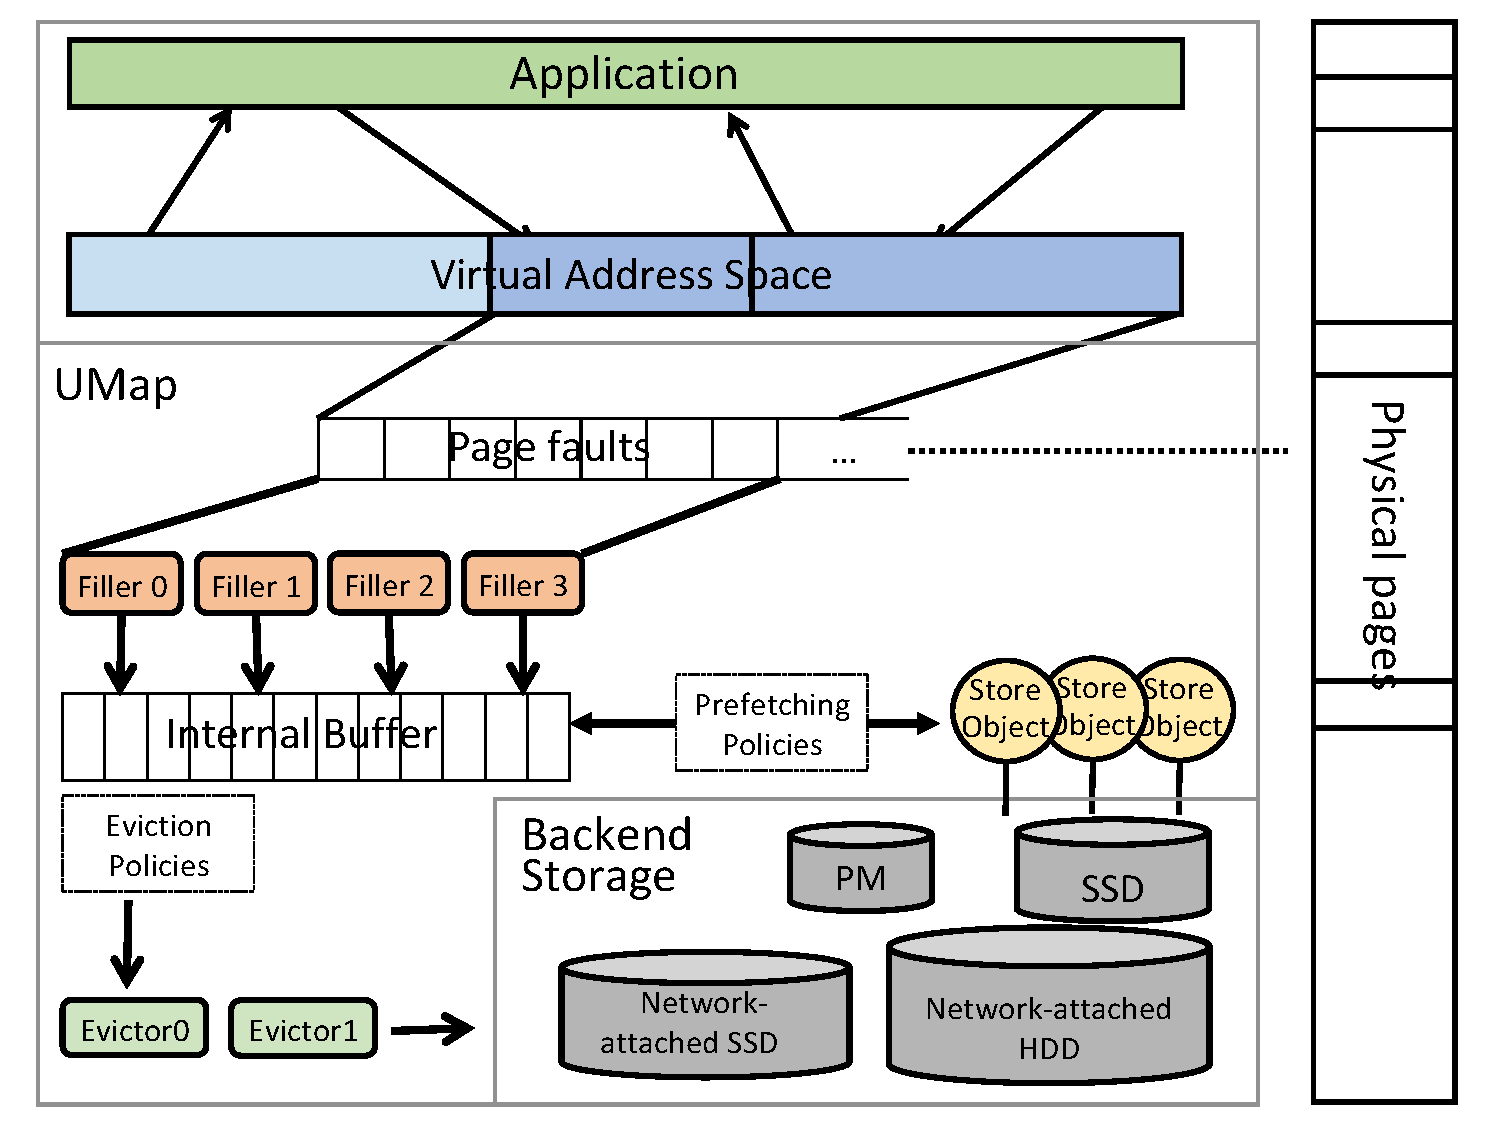
\includegraphics[scale = 0.5]{projects/2.3.1-PMR/2.3.1.19-Argo-PowerSteering/umap-arch}
        \caption{UMap Handler architecture}
        \label{fig:umaparch}
\end{figure}

\paragraph{Recent Progress}

In recent months, we have released UMap v2.1.0 and updated the UMap Spack package with major enhancements to improve load balancing and incorporate features for additional configurability. The new features include a SparseStore handler to optimize access to sparse, randomly accessed persistent data structures. The MetaAllocator Metall developed under the ECP SICM project has been integrated into UMap's SparseStore, enabling persistent heaps. 

UMap now supports a new network-based handler using the ECP Mochi data service to fetch and manage memory pages from remote nodes over the network. UMap also has a new capability to provide region-centric page access profiling from the collaboration with the ECP Caliper project. 

We have incorporated UMap into new applications, including the Livermore Metagenomics Toolkit (LMAT), which is being used for COVID research. We designed custom prefetching and eviction policies for LMAT.  The new solution outperforms the system solution in runtime by $5-15\%$ on realistic metagenomic queries and supports high parallelism that cannot be supported efficiently by the system solution. 

A paper on the UMap network handler has been accepted and presented at the IEEE SBAC-PAD 2020 conference. An SC20 poster on the UMap SparseStore handler is to appear.

\paragraph{Next Steps}
In the coming year, we plan to continue outreach to application teams
within ECP and in the science/data community. This includes
collaboration with Caliper, Mochi, Exagraph, the LMAT team, and
with LLNL users of materials and EOS tables. The Exagraph
collaboration will map persistent data such as binary format graphs
and intermediate data structures through UMap using the SparseStore
and Metall. To adapt to dynamic changes in memory resources, an adaptive buffer management will be added to monitor and react at runtime. To support the shared table use case, we will implement a multi-process version of UMap to be used by
multiple MPI processes on a node to share read-only tables stored in
persistent memory.

